\documentclass[border=6pt]{standalone}
\usepackage{tikz}
\usepackage{pgfplots}
\pgfplotsset{compat=1.18}
\usetikzlibrary{arrows.meta,positioning,shapes.geometric,fit,backgrounds,calc,decorations.pathreplacing,patterns}
\usetikzlibrary{pgfplots.groupplots}
\tikzset{
  blk/.style={rectangle, rounded corners=2pt, draw=black!70, thick, fill=blue!6,
              minimum height=8mm, minimum width=20mm, align=center, font=\small},
  io/.style={rectangle, rounded corners=6pt, draw=black!70, thick, fill=green!8,
             minimum height=8mm, align=center, font=\small},
  proc/.style={rectangle, draw=black!70, thick, fill=orange!10, minimum height=8mm,
               align=center, font=\small},
  dec/.style={diamond, aspect=2, draw=black!70, thick, fill=yellow!15, align=center, font=\footnotesize},
  warnbox/.style={rectangle, rounded corners=2pt, draw=red!60!black, thick, fill=red!7,
                  minimum height=8mm, align=center, font=\small},
  oklbox/.style={rectangle, rounded corners=2pt, draw=green!45!black, thick, fill=green!8,
                 minimum height=8mm, align=center, font=\small},
  ar/.style={-{Latex[length=2mm]}, thick},
  arl/.style={-{Latex[length=2mm]}, thick, dashed, draw=black!55},
  lbl/.style={font=\footnotesize\itshape, text=black!60},
}
\definecolor{good}{RGB}{34,139,34}
\definecolor{bad}{RGB}{178,34,34}
\definecolor{warn}{RGB}{218,165,32}
\definecolor{pesblue}{RGB}{0,45,98}
\definecolor{complete}{RGB}{30,125,79}
\definecolor{partial}{RGB}{176,106,0}
\definecolor{blocked}{RGB}{166,43,43}
\begin{document}
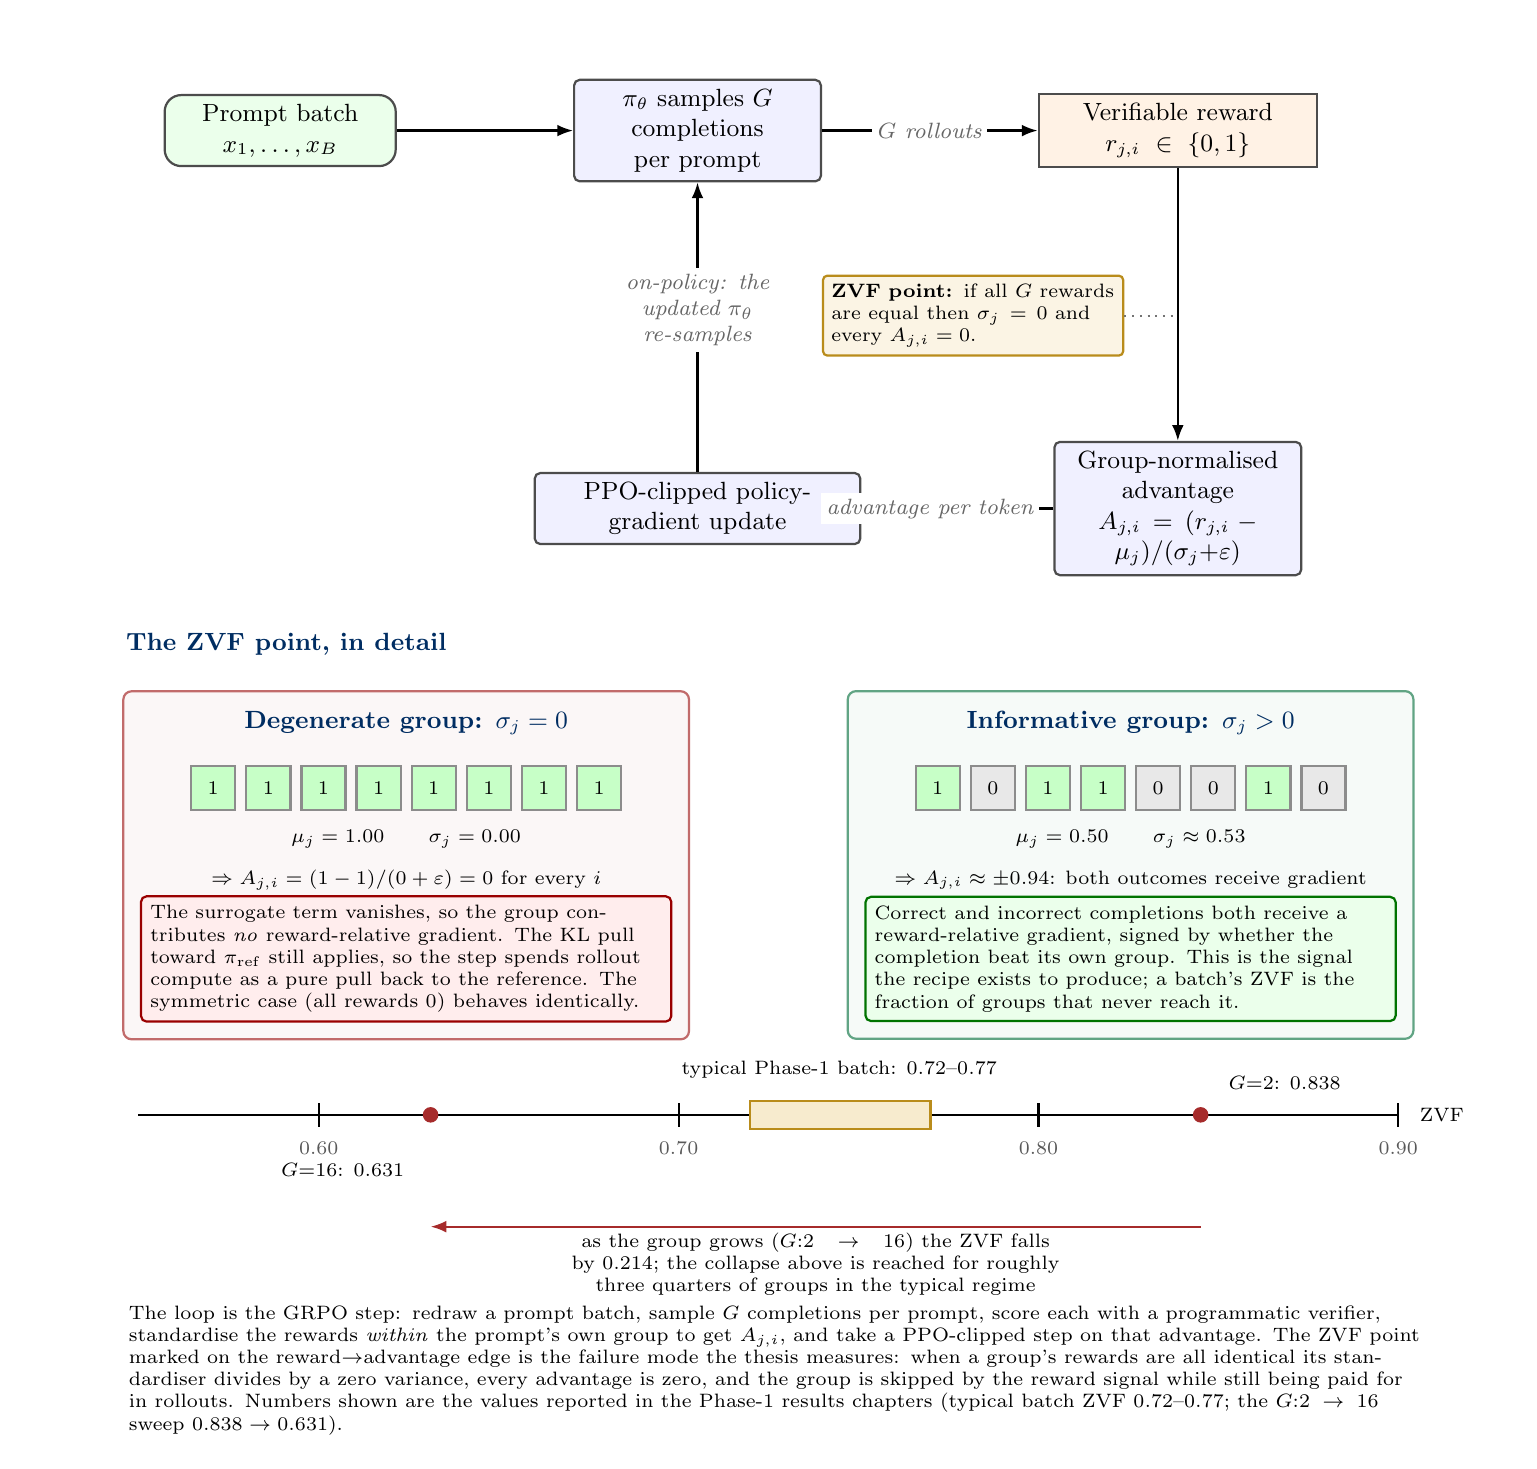
\begin{tikzpicture}[x=1cm,y=1cm,
  ion/.style={io, text width=2.7cm, font=\small},
  stn/.style={blk, text width=2.9cm, font=\small},
  pron/.style={proc, text width=3.3cm, font=\small},
  st/.style={blk, text width=3.9cm, font=\small},
  ch/.style={rectangle, draw=black!45, thick, minimum width=5.6mm, minimum height=5.6mm,
             inner sep=0pt, font=\scriptsize},
  c1/.style={ch, fill=green!22},
  c0/.style={ch, fill=black!9},
  hd/.style={font=\small\bfseries, text=pesblue, align=center, inner sep=1pt},
  stt/.style={font=\scriptsize, align=center, inner sep=1pt},
  stl/.style={font=\scriptsize, align=left, text width=16.4cm, inner sep=2pt},
  cardw/.style={draw=blocked!70, thick, rounded corners=3pt, fill=blocked!4, inner sep=6pt},
  cardg/.style={draw=complete!70, thick, rounded corners=3pt, fill=complete!4, inner sep=6pt},
  flagc/.style={rectangle, rounded corners=1.5pt, draw=warn!85!black, thick, fill=warn!12,
                font=\scriptsize, align=left, text width=3.6cm, inner sep=3pt},
  band/.style={fill=warn!22, draw=warn!85!black, thick},
]
% invisible path: fixes the bounding box
\draw[opacity=0] (-9.4,4.2) rectangle (9.4,-12.7);

% ===================== TOP: the GRPO training loop =====================
\node[ion] (A) at (-6.2, 2.9)  {Prompt batch\\ $x_1,\dots,x_B$};
\node[stn] (B) at (-0.9, 2.9)  {$\pi_\theta$ samples $G$\\ completions per prompt};
\node[pron] (C) at (5.2, 2.9)  {Verifiable reward\\ $r_{j,i}\in\{0,1\}$};
\node[stn] (F) at (5.2,-1.9)   {Group-normalised\\ advantage\\
                                $A_{j,i}=(r_{j,i}-\mu_j)/(\sigma_j{+}\varepsilon)$};
\node[st]  (E) at (-0.9,-1.9)  {PPO-clipped policy-gradient update};

\draw[ar] (A) -- (B);
\draw[ar] (B) -- (C);
\draw[ar] (C) -- (F);
\draw[ar] (F) -- (E);
\draw[ar] (E) -- (B);

\node[lbl, fill=white, inner sep=2pt] at (2.05, 2.9) {$G$ rollouts};
\node[lbl, fill=white, inner sep=2pt, align=center, text width=2.3cm]
  at (-0.9, 0.62) {on-policy: the\\ updated $\pi_\theta$ re-samples};
\node[lbl, fill=white, inner sep=2pt] at (2.05,-1.9) {advantage per token};

% the ZVF point, marked on the reward -> advantage edge
\node[flagc] (zflag) at (2.6, 0.55)
  {\textbf{ZVF point:} if all $G$ rewards are equal then $\sigma_j=0$
   and every $A_{j,i}=0$.};
\draw[dotted, thick, draw=black!55] (zflag.east) -- (5.2, 0.55);

% ===================== BOTTOM: the ZVF point in detail =====================
\node[hd, anchor=west] at (-8.2,-3.62) {The ZVF point, in detail};

% ---- left card: degenerate group ----
\node[hd] (Lt) at (-4.6,-4.62) {Degenerate group: $\sigma_j = 0$};
\node[c1] (Lc1) at (-7.05,-5.45) {1};
\node[c1] (Lc2) at (-6.35,-5.45) {1};
\node[c1] (Lc3) at (-5.65,-5.45) {1};
\node[c1] (Lc4) at (-4.95,-5.45) {1};
\node[c1] (Lc5) at (-4.25,-5.45) {1};
\node[c1] (Lc6) at (-3.55,-5.45) {1};
\node[c1] (Lc7) at (-2.85,-5.45) {1};
\node[c1] (Lc8) at (-2.15,-5.45) {1};
\node[stt] (Ls) at (-4.6,-6.10) {$\mu_j = 1.00\qquad \sigma_j = 0.00$};
\node[stt] (La) at (-4.6,-6.62)
  {$\Rightarrow A_{j,i} = (1-1)/(0+\varepsilon) = 0$ for every $i$};
\node[warnbox, text width=6.5cm, font=\scriptsize, align=left] (Lw) at (-4.6,-7.62)
  {The surrogate term vanishes, so the group contributes \emph{no} reward-relative
   gradient. The KL pull toward $\pi_{\mathrm{ref}}$ still applies, so the step spends
   rollout compute as a pure pull back to the reference. The symmetric case (all rewards
   $0$) behaves identically.};
\begin{scope}[on background layer]
  \node[cardw, fit=(Lt)(Lc1)(Lc8)(Ls)(La)(Lw)] (CL) {};
\end{scope}

% ---- right card: informative group ----
\node[hd] (Rt) at (4.6,-4.62) {Informative group: $\sigma_j > 0$};
\node[c1] (Rc1) at (2.15,-5.45) {1};
\node[c0] (Rc2) at (2.85,-5.45) {0};
\node[c1] (Rc3) at (3.55,-5.45) {1};
\node[c1] (Rc4) at (4.25,-5.45) {1};
\node[c0] (Rc5) at (4.95,-5.45) {0};
\node[c0] (Rc6) at (5.65,-5.45) {0};
\node[c1] (Rc7) at (6.35,-5.45) {1};
\node[c0] (Rc8) at (7.05,-5.45) {0};
\node[stt] (Rs) at (4.6,-6.10) {$\mu_j = 0.50\qquad \sigma_j \approx 0.53$};
\node[stt] (Ra) at (4.6,-6.62)
  {$\Rightarrow A_{j,i} \approx \pm 0.94$: both outcomes receive gradient};
\node[oklbox, text width=6.5cm, font=\scriptsize, align=left] (Rw) at (4.6,-7.62)
  {Correct and incorrect completions both receive a reward-relative gradient, signed by
   whether the completion beat its own group. This is the signal the recipe exists to
   produce; a batch's ZVF is the fraction of groups that never reach it.};
\begin{scope}[on background layer]
  \node[cardg, fit=(Rt)(Rc1)(Rc8)(Rs)(Ra)(Rw)] (CR) {};
\end{scope}

% ---- ZVF axis strip ----
\draw[thick] (-8.0,-9.6) -- (8.0,-9.6);
\filldraw[fill=warn!22, draw=warn!85!black, thick] (-0.23,-9.42) rectangle (2.06,-9.78);
\foreach \vv/\xx in {0.60/-5.71, 0.70/-1.14, 0.80/3.43, 0.90/8.00}{
  \draw[thick] (\xx,-9.45) -- (\xx,-9.75);
  \node[font=\scriptsize, text=black!65] at (\xx,-10.02) {\vv};
}
\node[font=\scriptsize, anchor=west] at (8.15,-9.60) {ZVF};
\node[font=\scriptsize] at (0.90,-9.03) {typical Phase-1 batch: $0.72$--$0.77$};
\filldraw[blocked] (5.49,-9.60) circle (2.6pt);
\node[font=\scriptsize, anchor=west] at (5.72,-9.20) {$G{=}2$: $0.838$};
\filldraw[blocked] (-4.29,-9.60) circle (2.6pt);
\node[font=\scriptsize, anchor=east] at (-4.50,-10.30) {$G{=}16$: $0.631$};
\draw[-{Latex[length=2mm]}, thick, draw=blocked] (5.49,-11.02) -- (-4.29,-11.02);
\node[font=\scriptsize, align=center, text width=9.0cm] at (0.60,-11.50)
  {as the group grows ($G{:}2\to16$) the ZVF falls by $0.214$; the collapse above is
   reached for roughly three quarters of groups in the typical regime};

\node[stl, anchor=north west] at (-8.2,-11.95)
  {The loop is the GRPO step: redraw a prompt batch, sample $G$ completions per prompt,
   score each with a programmatic verifier, standardise the rewards \emph{within} the
   prompt's own group to get $A_{j,i}$, and take a PPO-clipped step on that advantage.
   The ZVF point marked on the reward$\rightarrow$advantage edge is the failure mode the
   thesis measures: when a group's rewards are all identical its standardiser divides by
   a zero variance, every advantage is zero, and the group is skipped by the reward
   signal while still being paid for in rollouts. Numbers shown are the values reported
   in the Phase-1 results chapters (typical batch ZVF $0.72$--$0.77$; the $G{:}2\to16$
   sweep $0.838\to0.631$).};

\end{tikzpicture}
\end{document}
